\chapter{Literature Review}\label{ch:LitRev}
\section{Introduction}\label{sec:LitRevIntro}
In this section a summary of the major advances in skyrmion research is given, as well as the beginnings of the essential theory describing magnetic skyrmions.

Section \ref{sec:MagSkyrmions} gives a brief historical overview of the skyrmion, starting from its conception as a solution in particle physics through to its current significance in condensed matter physics. The types of skyrmions which exist and their fundamental differences and similarities are covered in section \ref{subsec:TypesSkyrmions}, followed by a discussion of the types of materials in which these different types are found in section \ref{subsec:Materials}. These materials are roughly divided between the bulk materials which produce skyrmion lattices, and thin films or multilayers which can host individual skyrmions.

Section \ref{subsec:TopConsiderations} is intended as a brief overview of the mathematical concepts in topology necessary to explain the special stability of skyrmions. This is followed by section \ref{subsec:InteractionsGovSkyrmions} which covers the interactions which govern the stability of skyrmions in different materials and allow us to tailor materials to produce environments in which skyrmions are stable at temperatures and magnetic field values that are desired for their industrial application. 
Section \ref{subsec:Anisotropies} introduces the idea of magnetic anisotropies, where they come from and the role which they can play in determining the magnetic properties of bulk materials, thin films and multilayers.

Section \ref{sec:AdvancesSkyrmionTech} concludes the literature review with some of the most significant recent advances including methods for nucleation of skyrmions, the dynamics of skyrmions and the environments necessary for their motion, the Skyrmion Hall Effect, and the potential applications of skyrmions in technology (\ref{subsec:Applications}).

\section{Magnetic Skyrmions}\label{sec:MagSkyrmions}
The word skyrmion generally refers to topologically protected defects in continuous non-linear fields which were first considered by Tony Skyrme in 1962.\cite{Skyrme1962} He considered that these defects, or multidimensional solitons, might behave as particles and that he might be able to thus create a field theory describing mesons and baryons. Despite the origin of skyrmions in particle physics the theory has now been applied to a wide variety of other areas of physics where field theories are essential to explaining phenomena. Most notable is the area of condensed matter physics where  skyrmion theory has been applied to various quantum hall and superconductivity theories\cite{Rho2016}, as well as liquid crystals \cite{Wright1989} and Bose-Einstein condensates.\cite{AlKhawaja2001,Brey1995}
Magnetic skyrmions are nano-sized magnetic structures which occur in a variety of different magnetic materials.\cite{Fert2017} Their existence in thin films and magnetic multilayers was first predicted in 2001 by Bogdanov and Ro{\ss}ler\cite{Bogdanov2001} and subsequently observed in 2011 by Heinze et. al.\cite{Heinze2011} in a one-atom layer of iron (Fe) on an iridium (Ir(111)). The skyrmions present in this material were found to be magnetic ground state of the monolayer of Fe on Ir, arranged spontaneously in a two-dimensional square lattice. Materials capable of hosting a skyrmion lattice briefly discussed in section \ref{subsec:Materials}. Individual skyrmions have also been observed in thin multilayers which exhibit an interfacial Dzyaloshinskii-Moriya interaction (DMI)\cite{Moriya1960, Dzyaloshinskii1958} due to interfacial symmetry breaking at heavy metal/ferromagnet/insulator layers and, importantly, have been shown to form using a driving current which introduces  spin transfer torque (STT).\cite{Jiang2015} The type of skyrmion present in different materials is highly dependent upon the form and origin of the DMI, this will be discussed in detail in sections \ref{subsec:SkyrmionType} and \ref{subsubsec:DMI}.

    \subsection{Skyrmion Definition}\label{subsec:SkyrDefn}

    \subsection{Types of Skyrmions}\label{subsec:TypesSkyrmions}
    \emph{Bloch Skyrmions}\label{subsec:Bloch} are defined by circular domain wall in which the magnetisation direction rotates from one direction at the perimeter to the opposite in the centre, whilst in plane magnetisation always points tangentially to the domain wall, as shown in figure \ref{fig:SkyrmionTypes} (a). These types of skyrmions are most commonly found as lattices in materials with the bulk DMI including MnSi and other B20 materials which have chiral crystal structure.\cite{Muhlbauer2009,Schulz2012}
    \emph{N\'{e}el Skyrmions} \label{subsec:Neel} are defined similarly to Bloch skyrmions however, they differ in that the magnetisation rotates from up to down whilst the in plane component of the magnetisation always points in a direction parallel or antiparallel to the skyrmion radius, as shown in figure \ref{fig:SkyrmionTypes} (b). N\'{e}el type skyrmions are most commonly observed in materials formed of magnetic multilayers where there is a large perpendicular magnetic anisotropy (PMA). The PMA draws the magnetisation of the material up out of the plane of the layers and this along with an additive in plane DMI leads to magnetisation that points radially through the skyrmion.

    \begin{figure}[t]
        \centering
           \subfigure[]{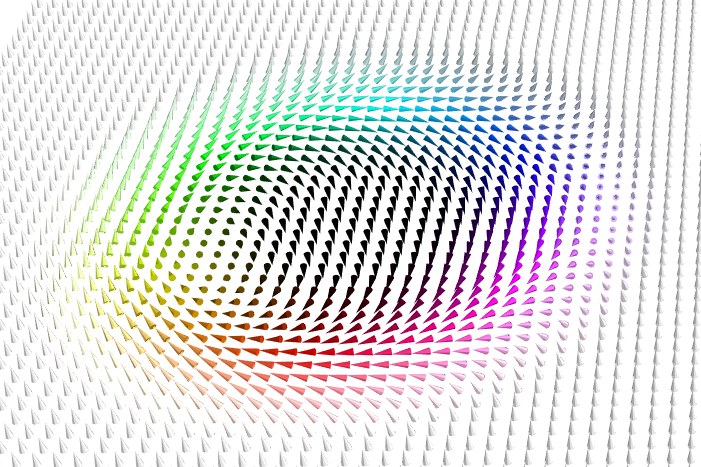
\includegraphics[width=.45\columnwidth]{BlochSkyrmion.png}}
           \subfigure[]{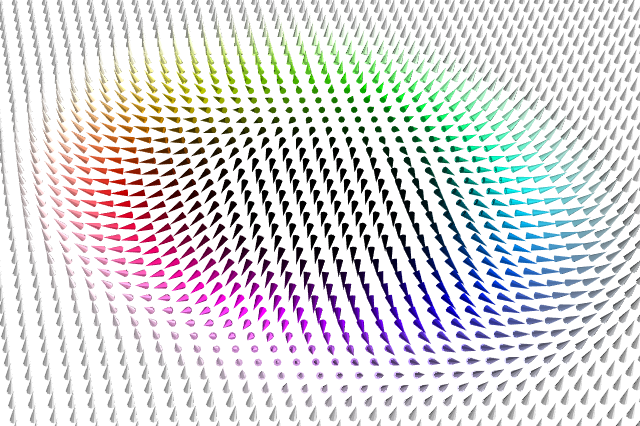
\includegraphics[width=.45\columnwidth]{NeelSkyrmion.png}}
           \caption{Types of Skyrmion: (a) A Bloch type skyrmion; (b) A N\'{e}el type skyrmion.
           Both types of skyrmion have magnetisation pointing upwards along the z axis around their perimeter and downwards along the z axis in their centres. In between these edge of the skyrmion and the centre there exists a finite, circular domain wall which is either (a) Bloch or (b) N\'{e}el.}
            \label{fig:SkyrmionTypes}
    \end{figure}

    \subsection{Materials Hosting Skyrmions}\label{subsec:Materials}
    Understanding the types of materials which can host different types of skyrmions is very important for any eventual application to industry. It is also an important consideration for this project which involves the design and fabrication of devices which will enable the investigation of electrical transport properties of skyrmions. In this section I will mainly emphasise the difference between materials in which 2D skyrmion lattices occur, spontaneously or in the presence of magnetic field, versus materials in which individual skyrmions are both present and stabilised. The main difference between these two groups is that skyrmion lattices occur mainly in bulk materials and individual skyrmions are observed in various types of multilayer however both types require a DMI to stabilise them. In bulk materials which occur as a cubic B20 crystals lacking inversion symmetry, such as MnSi, it was shown that the DMI was responsible for these observed helical magnetic structures\cite{Bak1980}.

    \subsection{Topological Considerations}\label{subsec:TopConsiderations}
    Skyrmions are defined by the mapping of their magnetisation directions, shown in Figure \ref{fig:SkyrmionTypes} (b), onto a sphere. One pole of the sphere represents the outside of the skyrmion and the other its centre, resulting in a sphere with arrows pointing outwards radially at all points in the case of a N\'{e}el skyrmion, as shown in Figure \ref{fig:spheremappings}\cite{Everschor-Sitte2014}. The mapping of the Bloch skyrmion magnetisation onto the surface of a sphere is also possible. This topology is defined by the skyrmion winding number, S, which indicates the integer number of `twists' in magnetisation texture of a skyrmion.
	
    \begin{equation}
        S=\frac{1}{4\pi}\int \textbf{M} \cdot \left( \frac{\partial \textbf{M}}{\partial x} \times \frac{\partial \textbf{M}}{\partial y}\right) \partial x \partial y 
    \end{equation}

    The fact that the skyrmion winding number cannot be changed by a continuous variation of the local magnetisation of the skyrmion is the cause of its enhanced stability relative to topologically trivial domain walls.
	 
    \begin{figure}[htbp]
	    \centering
	    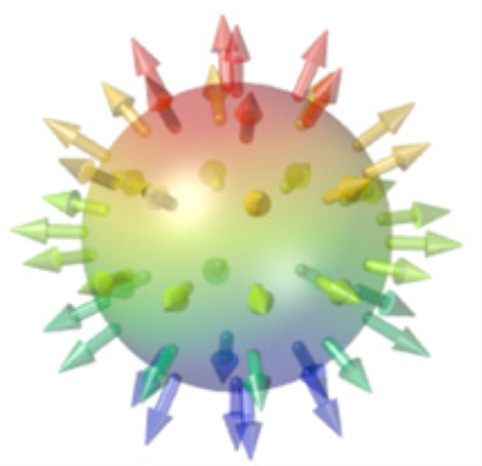
\includegraphics[width=0.25\columnwidth]{SphereMapping.png}
	    \caption{The local magnetisation of a N\'{e}el skyrmion mapped onto the surface of a sphere.\cite{Everschor-Sitte2014}}
	    \label{fig:spheremappings}
    \end{figure}

    \subsection{Anisotropies in Magnetism}\label{subsec:Anisotropies}
    Anisotropies are essentially asymmetries which cause one state to be more energetically favourable than another and must be taken into account in order to understand how non-collinear magnetic structures, for example skyrmions, could be supported in a material. Anisotropy is the general name given to the preference of a ferromagnetic material to maintain it's magnetisation in a particular direction or plane relative to the sample as a whole. This occurs due to an energy cost associated with the rotation of the magnetisation into certain axes. The energy cost is related to multiple sources including: shape anisotropy which arises due to the shape of the magnet; magnetocrystalline anisotropy which is due to the spin-orbit interaction between the electrons  in the lattice and the crystal lattice as a whole \cite{Kittel2005}; and surface anisotropy which occurs at surfaces and interfaces due to the loss of symmetry at the boundaries of a material. Understanding the interplay between anisotropies and the interactions discussed in section \ref{subsec:Interactions} allows us to tailor the materials used for device fabrication in order to have the best environment in which to create and measure skyrmions.

        \subsubsection*{Shape Anisotropy}
        Shape anisotropy occurs due to the shape of the magnet. This energy cost can be quantified by considering the magnetostatic energy of a dipole in an external field:
		\begin{equation}\label{eq:magnetostaticenergy}
			E=-\dfrac{\mu_{0}}{2}\int \textbf{M}\cdot\textbf{H} dV,
		\end{equation}
		where \textbf{M} is the magnetisation of the sample, \textbf{H} is the total internal field in the sample, and V is the volume of the magnetic sample. The internal field of the sample is the sum of the external field and the demagnetising field of the sample,
		\begin{equation}\label{eq:internalfield}
			\textbf{H}=\textbf{H}_{ext} + \textbf{H}_{d},
		\end{equation}
		where $\textbf{H}_{ext}$ is the external field, and $\textbf{H}_{d}$ is the demagnetising field. For the special case of ellipsoids the demagnetising field is proportional to the magnetisation of the sample, 
		\begin{equation}\label{eq:demagfactor}
			\textbf{H}_{d}=-N\textbf{M},
		\end{equation}
		where \emph{N} is a geometry dependent demagnetising factor. From this we can see that the magnetostatic energy will be higher when the sample is oriented to increase the demagnetising factor. The aim of minimising this energy promotes either single domain ferromagnets or domain orientations which minimise the overall energy due to the demagnetising, or stray, field of a magnet.
		
		\subsubsection*{Magnetocrystalline Anisotropy}\label{subsubsec:ShapeAni}
		Magnetocrystalline anisotropy is an intrinsic property of ferromagnetic materials. To first order it occurs due to spin-orbit interaction between each individual orbital electron's spin and the potential of the crystalline lattice. Spin-orbit coupling couples the spin of an electron with the magnetic field produced by it's motion, it can be described by the Hamiltonian of an effective spin-orbit field which acts on the individual orbital moments,
		\begin{equation}\label{eq:SOHamilitonian}
			\mathcal{H}_{SO}=-m_{1}\cdot\textbf{H}_{\text{eff SO}},
		\end{equation}
		where $m_{1}$ is the orbital moment and $\textbf{H}_{\text{eff SO}}$,
		\begin{equation}\label{eq:effSOfield}
			\text{H}_{\text{eff SO}} = \dfrac{-e\hbar^{2}\hat{\textbf{M}}}{4m_{e}^{2}c^{2}r\mu_{B}},
		\end{equation}
		is the effective spin-orbit field. In equation \ref{eq:effSOfield} $\hat{\textbf{M}}$ is the unit vector of the magnetisation of the sample. The main point to take away from this is that due to spin-orbit interaction between individual orbital moments and the overall crystalline lattice there will be energetically preferred crystalline axes. These are referred to as `easy' axes, the opposite which are energetically undesirable are called `hard' axes. The anisotropy field, $\textbf{H}_{a}$, is defined to be the field required to saturate the magnetisation of a crystal along it's hard axis\cite{Coey2009}, and is given by
		\begin{equation}
			\text{H}_{a}=\dfrac{2K_{eff}}{\mu_{0}M_{S}},
		\end{equation}
		where $K_{u}$ is the uniaxial anisotropy constant, M is the saturation magnetisation and t is the thickness of the sample.
		
		\subsubsection*{Surface Anisotropy}
		Surface anisotropy comes about due to the symmetry breaking of surfaces or interfaces between different types of magnetic materials. This anisotropy was first described by N\'eel in 1954\cite{Neel1954}. The loss of symmetry means that the anisotropy constants used to describe the magnetocrystalline anisotropy, $K_{V}$, must be adjusted to take account of the surface, $K_{S}$.
		
		\subssubsection*{Total Anisotropy Energy}
		The overall anisotropy energy of a thin film can be expressed as the sum of the energies due to the three types of anisotropy discussed above, 
		\begin{equation}\label{eq:anisotropyenergy}
			\begin{split}
			\text{E}_{ani}&=\text{E}_{uni}+\text{E}_{S}+\text{E}_{V}\\
			\text{K}\sin^{2}\Theta&=\left(-\mu_{0}\text{M}^{2} +\dfrac{2\text{K}_{S}}{t}+\text{K}_{V}\right)\sin^{2}\Theta.
			\end{split}
		\end{equation}
		
		\subsubsection*{Perpendicular Magnetic Anisotropy}\label{subsubsec:PMA}
		Perpendicular magnetic anisotropy (PMA) is the term used to describe a magnetic material which has an overall anisotropy which causes the magnetisation of the material to point perpendicular to the plane of the material. This effect is due to the combination of the anisotropies described above, as well as the DMI which was discussed in section \ref{subsubsec:DMI}.

        \subsubsection*{Demagnetising Anisotropy}\label{subsubsec:DemagAni}
        \begin{equation}
            K_{demag}=\dfrac{1}{2}\mu_{0}M^{2}_{S},
        \end{equation}
        where $M_{S}$ is the hard axis saturation magnetisation and $\mu_{0}$ is the permeability of free space.

        \subsubsection*{Effective Anisotropy}\label{subsubsec:EffAni}
        \begin{equation}
            K_{eff}=\dfrac{1}{2}\mu_{0}H_{S}M_{S},
        \end{equation}
        where $H_{S}$ and $M_{S}$ are the hard axis saturation field and magnetisation respectively and $\mu_{0}$ is the permeability of free space.

        \subsubsection*{Uniaxial Anisotropy}\label{subsubsec:UniAni}
        \begin{equation}
            K_{U}=K_{eff}+K_{demag}
        \end{equation}

    \subsection{Interactions Governing Skyrmion Stability}\label{subsec:InteractionsGovSkyrmions}

    \subsection*{Dipole-Dipole Interaction}\label{subsec:DipoleInt}

    \subsection*{Heisenberg Exchange Interaction}\label{subsec:ExchangeInt}

    \subsection*{Dzyaloshinskii-Moriya Interaction (DMI)}\label{subsec:DMI}
    \begin{figure}[htbp]
	    \centering	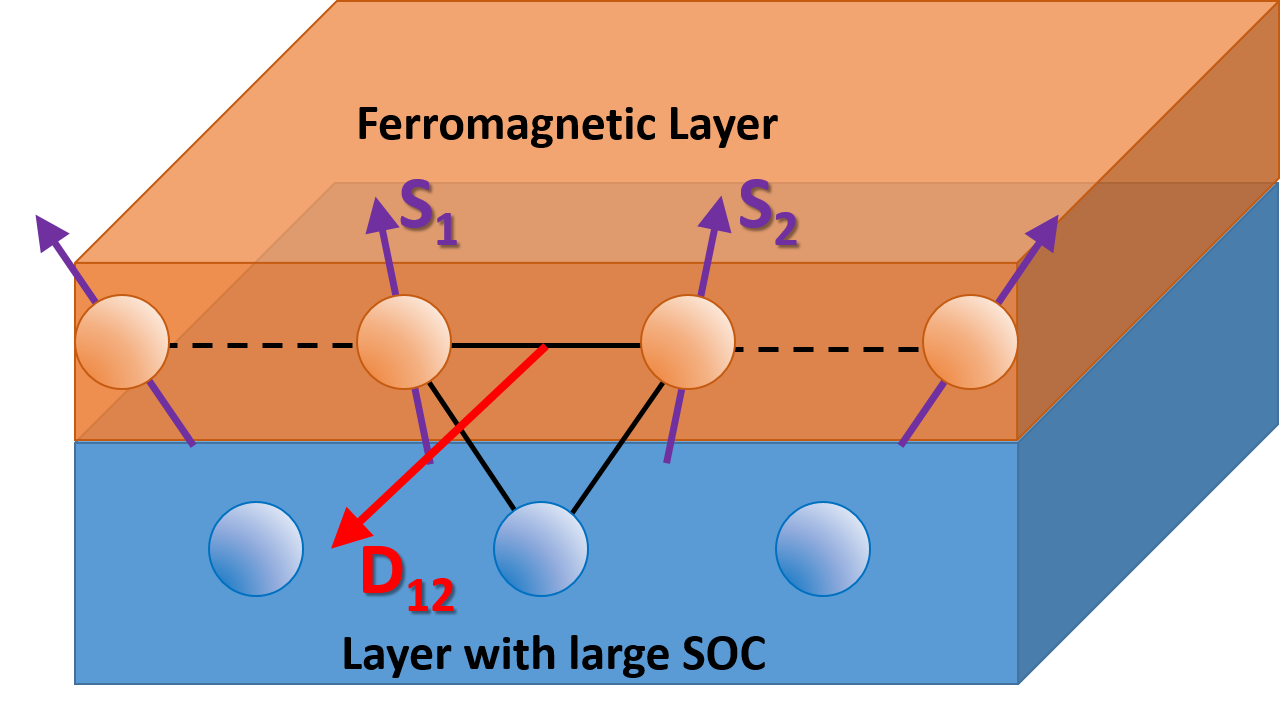
\includegraphics[width=0.4\columnwidth]{DMISchematic.png}
	    \caption{The interfacial DMI between a ferromagnetic layer and a layer of a material with a large spin orbit coupling.}
	    \label{fig:DMISchematic}
    \end{figure}
    Anisotropic exchange interactions occur in materials with a crystal structure that lacks inversion symmetry. The Dzyaloshinkii-Moriya Interaction is an example of such an interaction, named for Dzyaloshinskii who proposed the interaction in 1957\cite{Dzyaloshinskii1958} and Moriya who calculated the interaction for material systems including $\alpha$-Fe$_{2}$O$_{3}$, MnCO$_{3}$, and CrFe$_{3}$ in 1960\cite{Moriya1960}. An important aspect of the DMI is that it occurs when inversion symmetry is broken and as such it was suggested that DMI might be observable at the surface of a magnetic material,\cite{Fert1991}. This was confirmed analytically in 1998 by Crepieux and Lacroix \cite{Crepieux1998} who used mechanisms suggested by Moriya \cite{Moriya1960}, a microscopic model for localised magnetic systems, and Fert \& Levy \cite{Levy1981}, a three-site mechanism like the one shown in Figure \ref{fig:DMISchematic}, to calculate the DMI vector, $\emph{D}_{ij}$. The direction of $\emph{D}_{ij}$ was found for nearest neighbour sites at the surface and in the bulk for structures with simple cubic, BBC, and FCC lattices with different crystal planes as the surfaces in question.\cite{Crepieux1998} Nearly ten years later the effect of interfacial DMI on the chirality of magnetic structures was observed experimentally in a Mn monolayer on W(110), which used spin-polarised scanning tunneling microscopy to resolve the chirality of magnetic order within the Mn layer.\cite{Bode2007} The DMI has been shown to fix the chirality of domain walls and other structures, including skyrmions, throughout the material that it acts within. \cite{Heide2008,Benitez2015} In 2013 Je et al. included DMI and Zeeman energy terms in existing domain wall energy density formulae\cite{Lemerle1998,Kim2009} in order to analytically explore the properties of asymmetric bubble domain expansions in a Pt$\lvert$Co$\lvert$Pt trilayer.

    Figure \ref{fig:DMISchematic} illustrates the mechanism of the DMI suggested by Fert \& Levy, and is described by the Hamiltonian,
    \begin{equation}
	    \mathcal{\hat{H}}_{DMI}=\boldsymbol{D_{12}}\cdot\boldsymbol{S}_{1}\times\boldsymbol{S}_{2},
    \end{equation}
    where $\boldsymbol{D_{12}}$ is the DMI vector, and  $\boldsymbol{S}_{1}$ and $\boldsymbol{S}_{2}$ are the spin vectors of the two ferromagnetic ions. This mechanism is particularly applicable to the samples used throughout this project which are thin multilayers and have an interfacial DMI. This type of DMI acts between ions in a ferromagnetic layer of material and is mediated through spin orbit coupling with atoms in an adjacent layer. The layer adjacent to the ferromagnetic layer has the essential property of a large spin orbit coupling, allowing atoms near the interface to mediate the DMI.  This interaction acts to try to align the two spin vectors in a plane perpendicular to the DMI vector. In most cases the Heisenberg Hamiltonian is much larger than the DMI and as such the effect of the DMI is to slightly rotate the spins involved away from the ordering favoured by the exchange interaction.
	
\todo[inline]{\emph{DMI lit review} \\
\emph{Domain wall motion \& energy considerations} \\ 
\emph{Methods for measuring DMI include:} \\
- Spin polarised STM \cite{Meckler2009}\\
- Spin polarised low-energy electron microscopy \cite{Chen2013}\\
- Photoemission microscopy and XMCD \cite{Boulle2015}\\
*Expensive and time consuming\\
- Brillouin Light Scattering \cite{Nembach2015}\cite{Belmeguenai2015}\\

*Methods based on DW dynamics induced by magnetic fields:\\
- In flow regime use large IP field but deforms internatl structure of the DW which affects their dynamics \cite{Yamada2011}\\
- Asymmetric bubble expansion in creep regime \cite{Hrabec2014} \cite{Je2013}\\


\emph{Relation of IP H to DW velocity}
}

\section{Advances in Skyrmion Technology}\label{sec:AdvancesSkyrmionTech}
Initially Skyrmions were first observed as lattices in bulk and thin film materials, as discussed in Section \ref{subsec:SkyrmionIntro}. Individual Skyrmions were then observed soon afterwards in a PdFe bilayer by Romming et al.\cite{Romming2013}. Despite also showing that they could be manipulated in a controlled manner using spin-polarised tunnel currents this was only possible under quite specific conditions, at very low temperatures ($\approx$4K) and in the presence of an applied magnetic field ($\approx$1T) perpendicular to the surface of the material\cite{Romming2013}. Romming et al. also showed that the size and shape of individual magnetic Skyrmions was dependent on the magnetic field applied. By combining an analytical expression describing Skyrmions with experimental data they were able to show that careful experimental characterisation of the materials used can provide parameters, like DMI, which are responsible for the stability of individual Skyrmions\cite{Romming2015}. More recently individual skyrmions have been predicted\cite{Moreau-Luchaire2016} and observed at room temperature\cite{Woo2016,Boulle2016}, two conditions that are essential if skyrmions are ever to have widespread use in industry.

    \subsection{Skyrmion Dynamics}\label{subsec:Dynamics}

    \subsection{Potential Applications}\label{subsec:Applications}

    \subsection{The Hall Effect}\label{subsec:HallEffect}
    Despite the original discovery of the Hall effect in 1879 by Edward Hall, first for normal metals\cite{Hall1879}, and then in 1881 the larger effect which seen in ferromagnetic materials\cite{Hall1881}, it has taken well over one hundred years to establish a firm theoretical understanding and description of the latter. Hall observed that when a magnetic field is applied perpendicular to a current flowing within a conducting material, then a voltage is produced across that conductor, transverse to the direction of current flow\cite{Hall1879}. It is instructive to consider this effect in terms of the so called Hall resistivity ($\rho_{xy}$), or Hall conductivity ($\sigma_{xy}$), which expresses the ratio between the Hall voltage ($V_{H}$) and the current. This has allowed the overall phenomena seen in various types of materials to be broken down into the constituent Hall resistivities:

    \begin{equation}\label{eq:OverallHallResistivity}
    	\rho_{xy} = \rho_{xy}^{O} + \rho_{xy}^{A} + \rho_{xy}^{T},    
    \end{equation}
	
    which are attributed to separate physical phenomena. The overall Hall resistivity measured during experiments, $\rho_{xy}$, is given by the sum of the ordinary ($\rho_{xy}^{O}$), anomalous ($\rho_{xy}^{A}$), and topological ($\rho_{xy}^{T}$) Hall effects as shown in equation \ref{eq:OverallHallResistivity}.

        \subsubsection{Ordinary Hall Effect}\label{subsubsec:OHE}
        The ordinary Hall effect (OHE) was the first effect to be observed, in ordinary (non-magnetic) metals. By considering an experimental setup like the one shown in Figure \ref{fig:OHE} the effect can be explained simply by a qualitative understanding of the Lorentz force acting on the current flowing in the metal. Electrical current is the motion of charge carriers within a material, for a simple metal with electrons acting as charge carriers, the force experienced when moving in a magnetic field is given by the second term in
        \begin{equation}\label{eq:LorentzForce}
	        \textbf{F}= \textbf{F}_{E} + \textbf{F}_{B}  = q(\textbf{E}+\textbf{v}\times\textbf{B}),
        \end{equation}
        where $\textbf{E}$ is the electric field experienced by the charge carrier, q is the charge of that carrier, $\textbf{v}$ is the drift velocity of the charge carriers, and $\textbf{B}$ is the magnetic field experienced by the charge carriers. By virtue of the cross-product in equation \ref{eq:LorentzForce} it is possible to predict the direction of the Lorentz force using a right-hand rule where the thumb (\textbf{v} - velocity of electrons) , first finger (\textbf{B} - applied magnetic field), and second finger (\textbf{F}$_{B}$) take on the role of the three perpendicular vectors involved in the second term of the Lorentz force. Given this one should now expect the electrons to follow a path which curves towards one side of the material, according to the direction which the Lorentz force acts in, as shown in Figure \ref{fig:OHE}.
        \begin{figure}[t]
        	\centering
	        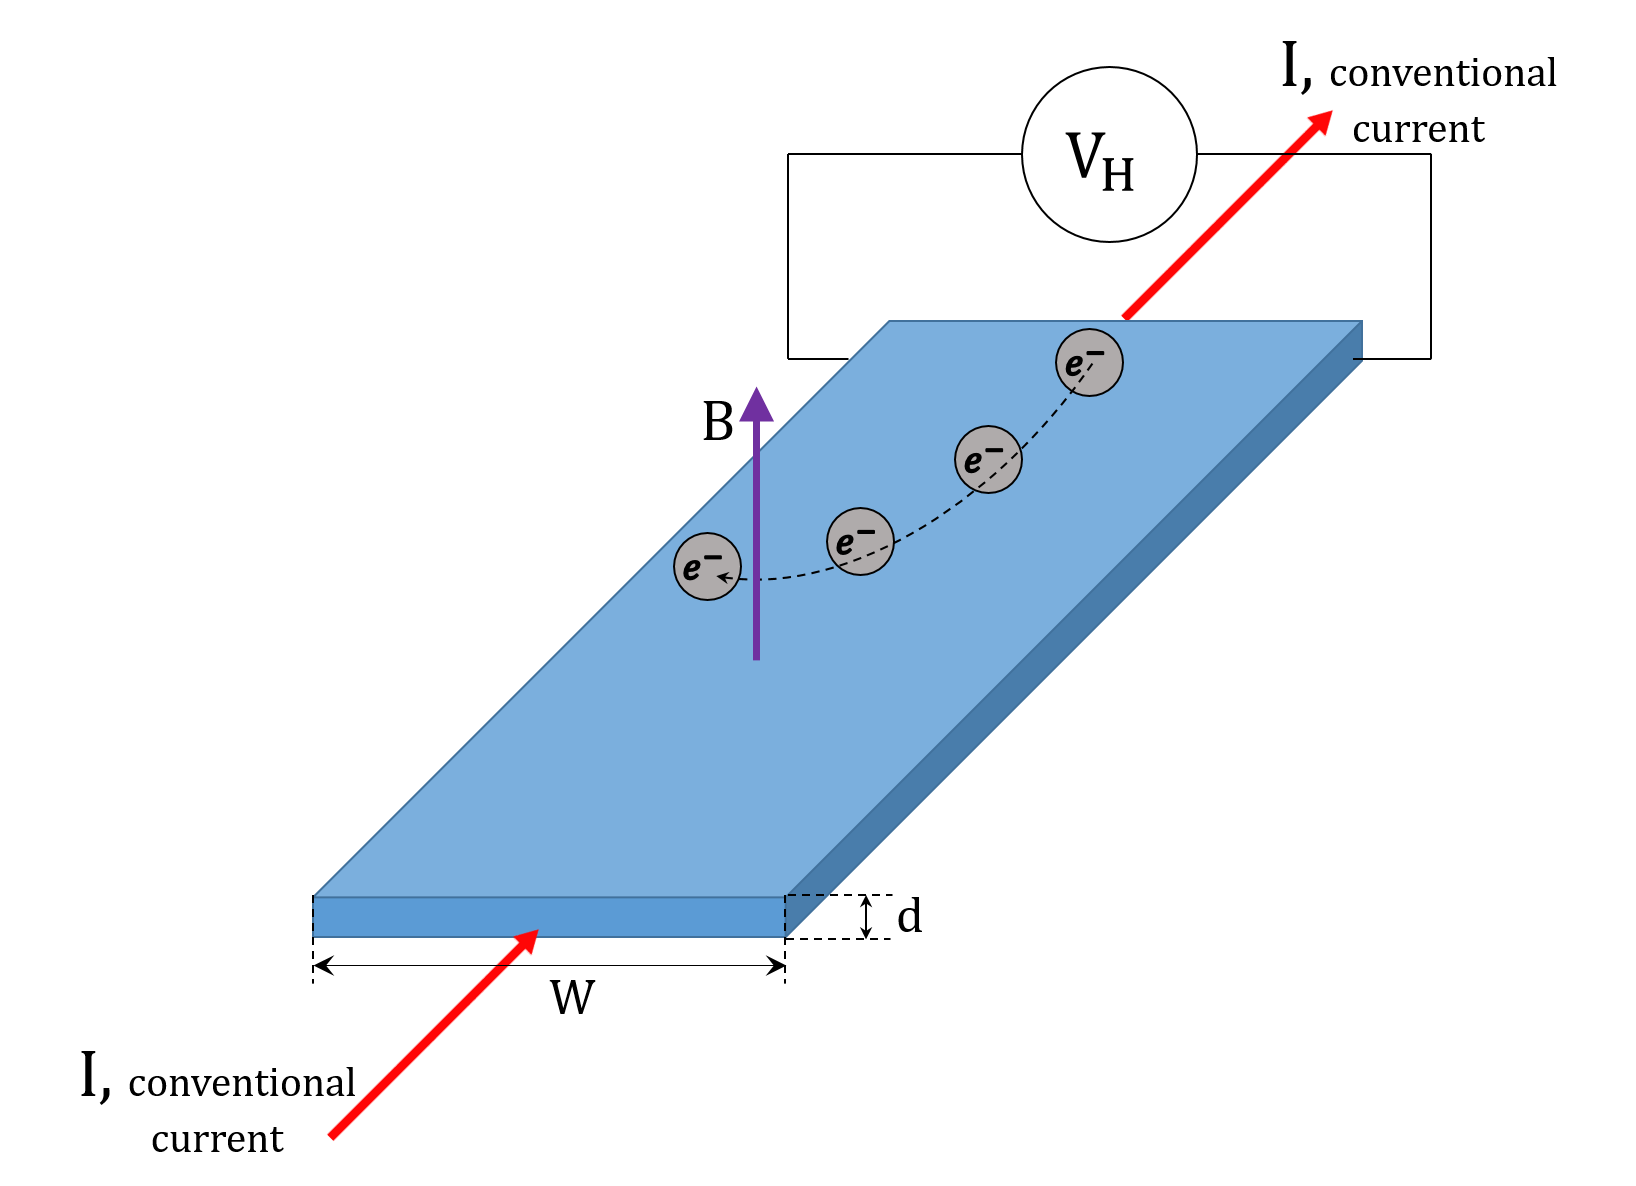
\includegraphics[width=0.5\columnwidth]{OrdinaryHallEffect.png}
    	    \caption{Schematic of an experimental arrangement to measure the ordinary Hall effect. The electrons follow a curved path to one side of the metal due to the Lorentz force from the external magnetic field, \textbf{B}. Note the electrons move with a velocity opposite to the direction of the conventional current.}
	        \label{fig:OHE}
        \end{figure}
        It was shown experimentally that the Hall resistivity for the OHE is proportional to the externally applied field,
        \begin{equation}\label{eq:OHE}
	       \rho_{xy}^{O} = R_{O}B,
        \end{equation}
        where $R_{O}$ is the ordinary Hall coefficient. The ordinary Hall coefficient is defined as
        \begin{equation}\label{eq:OHcoeff}
	        R_{O}=\dfrac{E_{y}}{j_{x}B}=\dfrac{V_{H}t}{IB},
        \end{equation}
        where $E_{y}$ is the induced electric field, $j_{x}=\dfrac{I}{t}$ is the current density, and B is the external field. $V_{H}$ is the Hall voltage which can be found by solving equation \ref{eq:LorentzForce} at equilibrium ($\textbf{F}=0$) to yield, 
        \begin{equation}\label{eq:hallvoltage}
	        V_{H}=\dfrac{I_{x}B_{z}}{nte},
        \end{equation}
        where $n$ is the charge carrier density, $t$ is the sample thickness, and $e$ is the magnitude of the charge of the electron.

        \subsubsection{Anomalous Hall Effect}\label{subsubsec:AHE}
        Ferromagnetic materials were observed to have a much larger Hall signal than normal metals shortly after the OHE in 1881\cite{Hall1881}. This came to be known as the anomalous Hall effect (AHE) and is was shown experimentally early on that the extra Hall resistivity seen in ferromagnetic materials could be described by
        \begin{equation}\label{eq:AHE}
    	    \rho_{xy}^{A} = R_{S}\mu_{0}M_{z},
        \end{equation}
        where $R_{S}$ is the anomalous Hall coefficient, and $M_{z}$ is the out-of-plane magnetisation of the sample\cite{Pugh1953}. However until recently the physical mechanisms behind the phenomenon have remained a mystery. In 1954 Karplus and Luttinger showed that it was possible to understand the AHE as the effect of spin-orbit interaction of polarised electrons\cite{Karplus1954}. An intrinisic mechanism of the AHE was first explained by Ye et al. considering colossal magnetoresistance manganites who showed that what had been observed was due to Berry phase effects due to carrier hopping in a non-trivial spin background\cite{Ye1999}. Even more recently in 2006, Onoda et al. presented a theory of the AHE which united the intrinsic contribution due spin-orbit coupling, and the extrinsic contribution due to `skew-scattering' of electrons due to an effective spin-orbit coupling with an impurity in the material, including the limits in which each contribution acts or dominates\cite{Onoda2006}. They also considered the extrinsic contribution due to `side-jumping' which occurs  when an electron's velocity is deflected in opposite directions by the opposite electric fields that it feels when approaching and moving away from an impurity\cite{Nagaosa2010}.

        \subsubsection{Topological Hall Effect}\label{subsubsec:THE}
        The Topological Hall Effect (THE) is the contribution to the overall Hall Effect due to topologically non-trivial magnetic textures like skyrmions\cite{Nagaosa2013}, in addition to the Ordinary Hall Effect (OHE) and the Anomalous Hall Effect (AHE).
        Current theory predicts that the topological Hall resistivity follows the following equation,
        \begin{equation}\label{eq:THE}
        	\rho_{xy}^{T} =  R_{0}PB_{eff}^{z},
        \end{equation}
        where P is the spin polarisation of the conduction electrons in the material, and $B_{eff}^{z}$ is the effective field which the electrons experience due to the Berry phase they gain whilst traversing the skyrmions\cite{Tanabe2017}. It was first distinguished by name from the AHE around fifteen years ago when it was shown by Bruno et al. that the topological Hall effect does not require any spin-orbit coupling contribution and can be explained purely by Berry phase theory of an electron moving through a smoothly varying magnetisation\cite{Bruno2004}. The THE was subsequently described in MnSi as due to the topologically non-trivial magnetisation of itinerant helimagnets in the B20 group\cite{Binz2008}. Recent work by Zeissler et. al. has observed a Hall signal with a characteristic dependence on the skyrmion winding number. That is a discrete contribution to the Hall resistivity due to N\'{e}el skyrmions present in a Hall disk, however the magnitude of the effect observed is much larger than that predicted by the existing Berry Phase theories for the THE\cite{Zeissler2018}. This project aims to improve the reliability of skyrmion nucleation, and combine this with Hall transport measurements in order to investigate the dependence of the topological Hall effect on skyrmion winding number, and understand the mechanism better, as it is clear the current theory may not be accounting for the whole picture. The THE has also been suggested as a possible method for skyrmion detection if they are to be used in industry for memory storage\cite{Hamamoto2016}. A complete understanding of the THE as well as reliable skyrmion nucleation and movement by all electrical means would be a huge step towards skyrmions finding a use in low energy magnetic memory devices.